\chapter{Leçon 29: Medien an Technologien}

Dës Lektioun beschäftegt sech mat de Froen an Äntwerten iwwer Medien an Technologien fir de Sproochentest. Mir analyséieren d'Medienlandschaft zu Lëtzebuerg, d'Gewunnechte vum Liesen, Tëlee kucken, Radio lauschteren, an den Internetgebrauch am Alldag. Mir widmen eis och der Wichtegkeet vun de sozialen Netzwierker an dem Handy am moderne Liewen. \textit{Cette leçon porte sur les questions et réponses concernant les médias et les technologies pour le Sproochentest. Nous analysons le paysage médiatique au Luxembourg, les habitudes de lecture, de télévision, de radio et l'utilisation d'Internet au quotidien. Nous abordons également l'importance des réseaux sociaux et du téléphone portable dans la vie moderne. / This lesson focuses on questions and answers about media and technologies for the Sproochentest. We analyze the media landscape in Luxembourg, habits of reading, watching TV, listening to the radio, and daily internet use. We also cover the importance of social networks and mobile phones in modern life.}

\vspace{1em}

\section[Froen an Äntwerten / Questions / Q\&A (Medien)]{Froen an Äntwerten: Medien an der Gesellschaft \\/ Questions et Réponses : Les médias dans la société \\/ Questions and Answers: Media in Society}

Hei ass eng ausféierlech Lëscht vu Froen an Äntwerten, déi Iech hëllefen, d'Medien an d'Technologie op Lëtzebuergesch ze beschreiwen. Fir all Fro ginn et zwou oder dräi méiglech Äntwerten mat verschiddene Formuléierungen an Detailer. \\
\textit{Voici une liste détaillée de questions et réponses pour vous aider à décrire les médias et la technologie en luxembourgeois. Pour chaque question, deux ou trois réponses possibles sont proposées avec différentes formulations et détails : / Here is a detailed list of questions and answers to help you describe media and technology in Luxembourgish. For each question, two or three possible answers are provided with different formulations and details:}

\vspace{1em}

\noindent\textbf{1. Wat fir Medië ginn et zu Lëtzebuerg?}\\
\textit{(Quels types de médias y a-t-il au Luxembourg ? / What kinds of media are there in Luxembourg?)}
\begin{itemize}
    \item \textbf{Äntwert A:} Zu Lëtzebuerg gëtt et vill verschidde Medien. Mir hunn national Zeitungen wéi d'Lëtzebuerger Wort an d'Tageblatt, an och eng populär Gratiszeitung wéi L'essentiel.\\
    \textit{Français : Au Luxembourg, il y a beaucoup de médias différents. Nous avons des journaux nationaux comme le Lëtzebuerger Wort et le Tageblatt, et aussi un journal gratuit populaire comme L'essentiel.}\\
    \textit{English : In Luxembourg, there are many different media. We have national newspapers like the Lëtzebuerger Wort and the Tageblatt, and also a popular free newspaper like L'essentiel.}
    \item \textbf{Äntwert B:} Et gëtt och vill digital Medien. De gréisste Sender fir Radio an Tëlee ass RTL Lëtzebuerg. Doniewent gëtt et vill online Portaler wéi reporter.lu oder virgule.lu.\\
    \textit{Français : Il y a aussi beaucoup de médias numériques. La plus grande chaîne de radio et de télévision est RTL Lëtzebuerg. En outre, il existe de nombreux portails en ligne comme reporter.lu ou virgule.lu.}\\
    \textit{English : There are also many digital media. The largest radio and TV station is RTL Lëtzebuerg. In addition, there are many online portals like reporter.lu or virgule.lu.}
    \item \textbf{Äntwert C:} Fir d'Leit, déi eng aner Sprooch schwätzen, gëtt et och auslännesch Medien an engleschsproocheg Säiten wéi Today.rtl.lu oder d'Luxembourg Times.\\
    \textit{Français : Pour les personnes qui parlent une autre langue, il y a aussi des médias étrangers et des pages en anglais comme Today.rtl.lu ou la Luxembourg Times.}\\
    \textit{English : For people who speak another language, there are also foreign media and English-language sites like Today.rtl.lu or the Luxembourg Times.}
\end{itemize}
\vspace{0.5em}

\noindent\textbf{2. Wéi oft liest Dir eng Zäitung?}\\
\textit{(À quelle fréquence lisez-vous un journal ? / How often do you read a newspaper?)}
\begin{itemize}
    \item \textbf{Äntwert A:} Ech liesen all Dag eng Zäitung. Moies beim Kaffi liesen ech gär d'Noriichten op mengem Handy fir ze wëssen, wat an der Welt an zu Lëtzebuerg geschitt.\\
    \textit{Français : Je lis un journal tous les jours. Le matin au petit-déjeuner, j'aime lire les nouvelles sur mon portable pour savoir ce qui se passe dans le monde et au Luxembourg.}\\
    \textit{English : I read a newspaper every day. In the morning at breakfast, I like to read the news on my phone to know what is happening in the world and in Luxembourg.}
    \item \textbf{Äntwert B:} Éierlech gesot liesen ech net oft eng gedréckt Zäitung. Ech liesen d'Noriichten éischter online oder op de soziale Medien, well dat méi séier a méi praktesch ass.\\
    \textit{Français : Honnêtement, je ne lis pas souvent de journal imprimé. Je lis plutôt les actualités en ligne ou sur les réseaux sociaux, car c'est plus rapide et plus pratique.}\\
    \textit{English : Honestly, I don't often read a printed newspaper. I read the news online or on social media instead, because it is faster and more convenient.}
    \item \textbf{Äntwert C:} Ech liesen eng Zäitung nëmmen um Weekend. Samschdes kafen ech d'Lëtzebuerger Wort fir d'Aktualitéit a Rou ze liesen, wann ech méi Zäit hunn.\\
    \textit{Français : Je ne lis un journal que le week-end. Le samedi, j'achète le Lëtzebuerger Wort pour lire l'actualité au calme quand j'ai plus de temps.}\\
    \textit{English : I only read a newspaper on weekends. On Saturdays, I buy the Lëtzebuerger Wort to read the news in peace when I have more time.}
\end{itemize}
\vspace{0.5em}

\noindent\textbf{3. Wat fir Rubricke liest Dir?}\\
\textit{(Quelles rubriques lisez-vous ? / What sections do you read?)}
\begin{itemize}
    \item \textbf{Äntwert A:} Ech liesen am léifsten d'Rubrik iwwer d'Lokalnoriichten an d'Politik, well ech mech dofir interesséieren, wat hei am Land lass ass.\\
    \textit{Français : Je préfère lire la rubrique des actualités locales et de la politique, car je m'intéresse à ce qui se passe dans le pays.}\\
    \textit{English : I prefer to read the section on local news and politics, because I am interested in what is going on in the country.}
    \item \textbf{Äntwert B:} Well ech e grousse Sportsfan sinn, liesen ech ëmmer als éischt d'Sportsrubrik fir d'Resultater vu Footballs- oder Cyclismusevenementer ze gesinn.\\
    \textit{Français : Comme je suis un grand fan de sport, je lis toujours en premier la rubrique sportive pour voir les résultats des événements de football ou de cyclisme.}\\
    \textit{English : Because I am a big sports fan, I always read the sports section first to see the results of football or cycling events.}
    \item \textbf{Äntwert C:} Ech liesen d'Kulturrubrik a d'Rezept-Iddien. Och d'Wiederprevisioun kucken ech mir ëmmer un, fir ze wëssen, wéi d'Wieder an den nächste Deeg gëtt.\\
    \textit{Français : Je lis la rubrique culturelle et les idées de recettes. Je regarde aussi toujours les prévisions météo pour savoir quel temps il fera dans les prochains jours.}\\
    \textit{English : I read the culture section and recipe ideas. I also always look at the weather forecast to know what the weather will be like in the coming days.}
\end{itemize}
\vspace{0.5em}

\noindent\textbf{4. Wat fir Zeitunge ginn et hei am Land?}\\
\textit{(Quels journaux y a-t-il dans le pays ? / What newspapers are there in this country?)}
\begin{itemize}
    \item \textbf{Äntwert A:} Zu Lëtzebuerg ginn et e puer grouss Zeitungen. Déi bekanntst ass d'Lëtzebuerger Wort. Et gëtt och d'Tageblatt an de Journal.\\
    \textit{Français : Au Luxembourg, il y a plusieurs grands journaux. Le plus connu est le Lëtzebuerger Wort. Il y a aussi le Tageblatt et le Journal.}\\
    \textit{English : In Luxembourg, there are several large newspapers. The most well-known is the Lëtzebuerger Wort. There is also the Tageblatt and the Journal.}
    \item \textbf{Äntwert B:} Fir d'Leit, déi mam Zuch oder dem Bus fueren, gëtt et d'Gratiszeitung L'essentiel op Franséisch. Déi läit bal an all Gare oder Bushaltestell.\\
    \textit{Français : Pour les personnes qui prennent le train ou le bus, il y a le journal gratuit L'essentiel en français. On le trouve dans presque toutes les gares ou arrêts de bus.}\\
    \textit{English : For people traveling by train or bus, there is the free newspaper L'essentiel in French. It can be found in almost every station or bus stop.}
    \item \textbf{Äntwert C:} Et ginn och Wochenzeitungen wéi de woxx oder d'Lëtzebuerger Land, déi méi déifgrënneg Analysen iwwer Politik an Economie maachen.\\
    \textit{Français : Il existe également des hebdomadaires comme le woxx ou d'Lëtzebuerger Land, qui proposent des analyses plus approfondies sur la politique et l'économie.}\\
    \textit{English : There are also weekly newspapers like woxx or d'Lëtzebuerger Land, which do more in-depth analyses of politics and economics.}
\end{itemize}
\vspace{0.5em}

\noindent\textbf{5. Liest Dir Zeitungen aus Ärem Heemechtsland? Kann ee se hei kafen?}\\
\textit{(Lisez-vous des journaux de votre pays d'origine ? Peut-on les acheter ici ? / Do you read newspapers from your home country? Can they be bought here?)}
\begin{itemize}
    \item \textbf{Äntwert A:} Jo, ech liesen reegelméisseg d'Zeitungen aus mengem Heemechtsland, awer nëmmen online. Dat ass méi einfach an ech muss se net am Buttek sichen.\\
    \textit{Français : Oui, je lis régulièrement les journaux de my pays d'origine, mais uniquement en ligne. C'est plus facile et je n'ai pas besoin de les chercher en magasin.}\\
    \textit{English : Yes, I regularly read newspapers from my home country, but only online. It is easier and I don't have to look for them in shops.}
    \item \textbf{Äntwert B:} Neen, ech liesen keng Zeitungen aus menger Heemecht méi. Ech konzentréieren mech elo op d'Lëtzebuerger Noriichten fir meng Sprooch ze verbesseren.\\
    \textit{Français : Non, je ne lis plus de journaux de ma patrie. Je me concentre maintenant sur les actualités luxembourgeoises pour améliorer ma langue.}\\
    \textit{English : No, I don't read newspapers from my homeland anymore. I now focus on Luxembourgish news to improve my language.}
    \item \textbf{Äntwert C:} Jo, heiansdo kafen ech eng Zäitung aus mengem Heemechtsland. Op der Gare an de grousse Kiosken kann een e puer international Zeitungen kafen.\\
    \textit{Français : Oui, j'achète parfois un journal de mon pays d'origine. À la gare, dans les grands kiosques, on peut acheter quelques journaux internationaux.}\\
    \textit{English : Yes, sometimes I buy a newspaper from my home country. At the train station in the large kiosks, you can buy some international newspapers.}
\end{itemize}
\vspace{0.5em}

\noindent\textbf{6. Liest Dir Zäitschrëften?}\\
\textit{(Lisez-vous des magazines ? / Do you read magazines?)}
\begin{itemize}
    \item \textbf{Äntwert A:} Normalerweis liesen ech keng Zäitschrëften, mee heiansdo maachen ech dat, wann ech beim Dokter am Waardesall sëtzen an op mäin Tour waarden.\\
    \textit{Français : Normalement, je ne lis pas de magazines, mais parfois je le fais quand je suis assis dans la salle d'attente du médecin et que j'attends mon tour.}\\
    \textit{English : Usually, I don't read magazines, but sometimes I do when I am sitting in the doctor's waiting room and waiting for my turn.}
    \item \textbf{Äntwert B:} Jo, ech liesen eng technologesch Zäitschrëft eemol am Mount, well dat mäin Hobby ass an ech gäre Neiegkeeten iwwer Computer an Apparater liesen.\\
    \textit{Français : Oui, je lis un magazine technologique une fois par mois, car c'est mon hobby et j'aime lire des nouveautés sur les ordinateurs et les appareils.}\\
    \textit{English : Yes, I read a technology magazine once a month, because it is my hobby and I like to read news about computers and devices.}
    \item \textbf{Äntwert C:} Neen, ech liesen eigentlech guer keng Zäitschrëften. Wann ech Fräizäit hunn, liesen ech léiwer e Buch oder kucken eng Serie.\\
    \textit{Français : Non, je ne lis en fait aucun magazine. Quand j'ai du temps libre, je préfère lire un livre ou regarder une série.}\\
    \textit{English : No, I actually don't read magazines at all. When I have free time, I prefer to read a book or watch a series.}
\end{itemize}
\vspace{0.5em}

\noindent\textbf{7. Abonéiert Dir eng Zäitung?}\\
\textit{(Êtes-vous abonné à un journal ? / Do you subscribe to a newspaper?)}
\begin{itemize}
    \item \textbf{Äntwert A:} Neen, ech hunn am Moment keng Zäitung abonéiert. Ech kafen heiansdo eng Zäitung am Kiosk oder liesen d'Noriichten gratis online.\\
    \textit{Français : Non, je n'ai pas d'abonnement à un journal en ce moment. J'achète parfois un journal au kiosque ou je lis les actualités gratuitement en ligne.}\\
    \textit{English : No, I do not subscribe to a newspaper at the moment. I sometimes buy a newspaper at the kiosk or read the news for free online.}
    \item \textbf{Äntwert B:} Jo, ech hunn en digitalen Abonnement fir d'Lëtzebuerger Wort. Dat ass méi bëlleg wéi d'Pabeierversioun an ech kann et iwwerall liesen.\\
    \textit{Français : Oui, j'ai un abonnement numérique pour le Lëtzebuerger Wort. C'est moins cher que la version papier et je peux le lire partout.}\\
    \textit{English : Yes, I have a digital subscription to the Lëtzebuerger Wort. It is cheaper than the paper version and I can read it anywhere.}
    \item \textbf{Äntwert C:} Jo, meng Famill huet zanter Joren e Pabeierabonnement. D'Zäitung gëtt eis all Moien direkt an d'Bréifkëscht geliwwert.\\
    \textit{Français : Oui, ma famille a un abonnement papier depuis des années. Le journal nous est livré chaque matin directement dans la boîte aux lettres.}\\
    \textit{English : Yes, my family has had a paper subscription for years. The newspaper is delivered directly to our mailbox every morning.}
\end{itemize}
\vspace{0.5em}

\noindent\textbf{8. Kaaft Dir Zäitungen? Wou kaaft Dir se?}\\
\textit{(Achetez-vous des journaux ? Où les achetez-vous ? / Do you buy newspapers? Where do you buy them?)}
\begin{itemize}
    \item \textbf{Äntwert A:} Ech kafen net oft Zäitungen. Wann ech awer eng kafen, maachen ech dat am Kiosk op der Gare oder an engem grousse Cactus-Supermarché.\\
    \textit{Français : Je n'achète pas souvent de journaux. Mais si j'en achète un, je le fais au kiosque de la gare ou dans un grand supermarché Cactus.}\\
    \textit{English : I don't buy newspapers often. But when I do buy one, I do it at the station kiosk or in a large Cactus supermarket.}
    \item \textbf{Äntwert B:} Neen, ech kafen ni Zäitungen. Ech liesen nëmmen déi gratis Online-Artikelen oder lauschteren d'Noriichten um Radio wärend der Aarbecht.\\
    \textit{Français : Non, je n'achète jamais de journaux. Je lis uniquement les articles gratuits en ligne ou j'écoute les nouvelles à la radio pendant le travail.}\\
    \textit{English : No, I never buy newspapers. I only read free online articles or listen to the news on the radio during work.}
    \item \textbf{Äntwert C:} Jo, ech kafen all Samschdeg eng Zäitung bei der Tankstell, wann ech den Auto tanke goen. Dat ass eng kleng Gewunnecht ginn.\\
    \textit{Français : Oui, j'achète un journal tous les samedis à la station-service quand je vais faire le plein de la voiture. C'est devenu une petite habitude.}\\
    \textit{English : Yes, I buy a newspaper every Saturday at the gas station when I go to fill up the car. It has become a little habit.}
\end{itemize}
\vspace{0.5em}

\noindent\textbf{9. Wéi oft kuckt Dir d’Tëlee?}\\
\textit{(À quelle fréquence regardez-vous la télévision ? / How often do you watch TV?)}
\begin{itemize}
    \item \textbf{Äntwert A:} Normalerweis kucken ech keng klassesch Tëlee. Ech kucken Streaming-Servicer wéi Netflix oder YouTube um Internet, wann ech Zäit hunn.\\
    \textit{Français : Normalement, je ne regarde pas la télévision classique. Je regarde plutôt des services de streaming comme Netflix ou YouTube sur Internet quand j'ai le temps.}\\
    \textit{English : Usually, I don't watch classic TV. I watch streaming services like Netflix or YouTube on the internet when I have time.}
    \item \textbf{Äntwert B:} Ech kucken all Owend eng Stonn Tëlee. Meeschtens kucken ech den RTL Journal fir ze gesinn, wat haut an eisem Land geschitt ass.\\
    \textit{Français : Je regarde la télévision une heure chaque soir. La plupart du temps, je regarde le journal de RTL pour voir ce qui s'est passé aujourd'hui dans notre pays.}\\
    \textit{English : I watch TV for an hour every evening. Mostly I watch the RTL Journal to see what happened in our country today.}
    \item \textbf{Äntwert C:} Ech kucken bal ni Tëlee. Ech liesen léiwer e Buch oder spillen e Gesellschaftsspill, dat ass vill méi gesond fir d'Aen.\\
    \textit{Français : Je ne regarde presque jamais la télé. Je préfère lire un livre ou jouer à un jeu de société, c'est beaucoup plus sain pour les yeux.}\\
    \textit{English : I almost never watch TV. I prefer to read a book or play a board game, which is much healthier for the eyes.}
\end{itemize}
\vspace{0.5em}

\noindent\textbf{10. Lauschtert Dir oft de Radio?}\\
\textit{(Écoutez-vous souvent la radio ? / Do you listen to the radio often?)}
\begin{itemize}
    \item \textbf{Äntwert A:} Jo, ech lauschteren all Dag Radio. Ech maachen de Radio direkt moies un, wann ech opstinn an de Kaffi preparéieren.\\
    \textit{Français : Oui, j'écoute la radio tous les jours. J'allume la radio dès le matin quand je me lève et que je prépare le café.}\\
    \textit{English : Yes, I listen to the radio every day. I turn on the radio first thing in the morning when I get up and prepare coffee.}
    \item \textbf{Äntwert B:} Neen, ech lauschtere selten de Radio. Ech lauschtere léiwer meng eegen Playlist op Spotify oder e Podcast, dee mech interesséiert.\\
    \textit{Français : Non, j'écoute rarement la radio. Je préfère écouter ma propre liste de lecture sur Spotify ou un podcast qui m'intéresse.}\\
    \textit{English : No, I rarely listen to the radio. I prefer to listen to my own playlist on Spotify or a podcast that interests me.}
    \item \textbf{Äntwert C:} Jo, ech lauschtere Radio beim Kachen oder beim Botzen. Dat mécht d'Hausaarbecht méi agreabel a manner langweileg.\\
    \textit{Français : Oui, j'écoute la radio en cuisinant ou en faisant le ménage. Cela rend les tâches ménagères plus agréables et moins ennuyeuses.}\\
    \textit{English : Yes, I listen to the radio while cooking or cleaning. That makes housework more pleasant and less boring.}
\end{itemize}
\vspace{0.5em}

\noindent\textbf{11. Wéini a wou lauschtert Dir de Radio?}\\
\textit{(Quand et où écoutez-vous la radio ? / When and where do you listen to the radio?)}
\begin{itemize}
    \item \textbf{Äntwert A:} Ech lauschtere Radio meeschtens moies fréi an der Kichen an och am Auto um Wee fir op d'Aarbecht an zréck heem.\\
    \textit{Français : J'écoute la radio la plupart du temps tôt le matin dans la cuisine et aussi dans la voiture sur le chemin du travail et du retour.}\\
    \textit{English : I listen to the radio mostly early in the morning in the kitchen and also in the car on my way to work and back home.}
    \item \textbf{Äntwert B:} Ech lauschtere Radio wärend der Aarbecht am Büro, mee ganz leis, fir meng Kollegen net ze stéieren. Dat hëlleft mir ze konzentréieren.\\
    \textit{Français : J'écoute la radio pendant le travail au bureau, mais très doucement, pour ne pas déranger mes collègues. Cela m'aide à me concentrer.}\\
    \textit{English : I listen to the radio during work in the office, but very quietly, so as not to disturb my colleagues. It helps me concentrate.}
    \item \textbf{Äntwert C:} Ech lauschtere Radio owes, wann ech am Bett leien an mech entspanen, meeschtens e Programm mat roueger Musek.\\
    \textit{Français : J'écoute la radio le soir quand je suis allongé dans mon lit et que je me détends, le plus souvent un programme de musique calme.}\\
    \textit{English : I listen to the radio in the evening when I lie in bed and relax, usually a program with quiet music.}
\end{itemize}
\vspace{0.5em}

\noindent\textbf{12. Wat fir Radiosendere ginn et zu Lëtzebuerg? Wat kennt Dir?}\\
\textit{(Quelles stations de radio y a-t-il au Luxembourg ? Lesquelles connaissez-vous ? / What radio stations are there in Luxembourg? Which ones do you know?)}
\begin{itemize}
    \item \textbf{Äntwert A:} Zu Lëtzebuerg ginn et e puer bekannt Radiosendere. De beléifsten ass RTL Radio Lëtzebuerg, deen Noriichten a vill Musek op Lëtzebuergesch bréngt.\\
    \textit{Français : Au Luxembourg, il y a plusieurs stations de radio connues. La plus populaire est RTL Radio Lëtzebuerg, qui diffuse des nouvelles et beaucoup de musique en luxembourgeois.}\\
    \textit{English : In Luxembourg, there are several known radio stations. The most popular is RTL Radio Lëtzebuerg, which brings news and a lot of music in Luxembourgish.}
    \item \textbf{Äntwert B:} Ech kennen den Eldoradio, dee vill modern Musek an Charts spillt. Fir international Leit gëtt et den Ara, deen Emissiounen a verschiddene Sproochen huet.\\
    \textit{Français : Je connais Eldoradio, qui joue beaucoup de musique moderne et de hits. Pour les internationaux, il y a Ara, qui a des émissions en plusieurs langues.}\\
    \textit{English : I know Eldoradio, which plays a lot of modern music and charts. For international people, there is Ara, which has programs in different languages.}
    \item \textbf{Äntwert C:} Et gëtt och den 100komma7, dat ass de kulturelle Radiosender, an och den L'essentiel Radio fir déi franséischsproocheg Leit.\\
    \textit{Français : Il y a aussi 100komma7, qui est la station de radio culturelle, et aussi L'essentiel Radio pour les personnes francophones.}\\
    \textit{English : There is also 100komma7, which is the cultural radio station, and also L'essentiel Radio for French-speaking people.}
\end{itemize}
\vspace{0.5em}

\noindent\textbf{13. Benotzt Dir oft den Internet?}\\
\textit{(Utilisez-vous souvent Internet ? / Do you use the internet often?)}
\begin{itemize}
    \item \textbf{Äntwert A:} Jo, ech benotzen den Internet bal de ganzen Dag. Souwuel fir meng Aarbecht wéi och a menger Fräizäit ass den Internet néideg.\\
    \textit{Français : Oui, j'utilise Internet presque toute la journée. Internet est nécessaire tant pour mon travail que pour mes loisirs.}\\
    \textit{English : Yes, I use the internet almost all day. The internet is necessary both for my work and in my free time.}
    \item \textbf{Äntwert B:} Jo, ech benotzen den Internet ganz oft, meeschtens op mengem Handy fir meng E-Mailen ze checken oder de Wee op Google Maps ze sichen.\\
    \textit{Français : Oui, j'utilise Internet très souvent, principalement sur mon portable pour vérifier mes e-mails ou chercher mon chemin sur Google Maps.}\\
    \textit{English : Yes, I use the internet very often, mostly on my phone to check my emails or look for directions on Google Maps.}
    \item \textbf{Äntwert C:} Ech benotzen den Internet reegelméisseg, mee ech probéieren owes meng Apparater auszeschalten, fir net ze vill Zäit online ze verbréngen.\\
    \textit{Français : J'utilise Internet régulièrement, mais j'essaie d'éteindre mes appareils le soir pour ne pas passer trop de temps en ligne.}\\
    \textit{English : I use the internet regularly, but I try to turn off my devices in the evening so as not to spend too much time online.}
\end{itemize}
\vspace{0.5em}

\noindent\textbf{14. Wéi vill Zäit verbréngt Dir pro Dag / pro Woch um Internet?}\\
\textit{(Combien de temps passez-vous sur Internet par jour / par semaine ? / How much time do you spend on the internet per day / per week?)}
\begin{itemize}
    \item \textbf{Äntwert A:} Ech verbrénge pro Dag ongeféier dräi bis véier Stonnen um Internet. Dës Zäit ass opgedeelt tëscht menger Aarbecht an de sozialen Netzwierker.\\
    \textit{Français : Je passe environ trois à quatre heures sur Internet par jour. Ce temps est partagé entre mon travail et les réseaux sociaux.}\\
    \textit{English : I spend about three to four hours on the internet per day. This time is split between my work and social networks.}
    \item \textbf{Äntwert B:} Well ech de ganzen Dag am Büro um Computer schaffen, verbrénge ech sécherlech méi wéi aacht Stonnen den Dag online. Dat ass vill.\\
    \textit{Français : Comme je travaille toute la journée au bureau sur ordinateur, je passe certainement plus de huit heures par jour en ligne. C'est beaucoup.}\\
    \textit{English : Since I work all day in the office on a computer, I certainly spend more than eight hours a day online. That is a lot.}
    \item \textbf{Äntwert C:} Pro Woch verbréngen ech ongeféier zwanzeg Stonnen um Internet. Ech probéieren mäi Konsum ze limitéieren, besonnesch um Weekend.\\
    \textit{Français : Par semaine, je passe environ vingt heures sur Internet. J'essaie de limiter ma consommation, surtout le week-end.}\\
    \textit{English : Per week, I spend about twenty hours on the internet. I try to limit my consumption, especially on weekends.}
\end{itemize}
\vspace{0.5em}

\noindent\textbf{15. Wat maacht Dir alles online?}\\
\textit{(Que faites-vous en ligne ? / What do you do online?)}
\begin{itemize}
    \item \textbf{Äntwert A:} Ech maachen vill online. Ech liesen d'Noriichten, kucke Videoen, bezuelen d'Rechnungen iwwer Homebanking an kafen heiansdo Saachen.\\
    \textit{Français : Je fais beaucoup de choses en ligne. Je lis les actualités, je regarde des vidéos, je paie les factures par banque en ligne et j'achète parfois des choses.}\\
    \textit{English : I do a lot online. I read the news, watch videos, pay bills via online banking, and sometimes buy things.}
    \item \textbf{Äntwert B:} Ech benotzen den Internet fir mat menger Famill ze chatten, Fotoen op Instagram ze deelen a meng nächst Reesen ze plangen.\\
    \textit{Français : J'utilise Internet pour discuter avec ma famille, partager des photos sur Instagram et planifier mes prochains voyages.}\\
    \textit{English : I use the internet to chat with my family, share photos on Instagram, and plan my next trips.}
    \item \textbf{Äntwert C:} Online liesen ech Artikelen iwwer meng Hobbien, ech léiere Lëtzebuergesch mat online Coursen an ech kucken d'Wieder.\\
    \textit{Français : En ligne, je lis des articles sur mes loisirs, j'apprends le luxembourgeois avec des cours en ligne et je regarde la météo.}\\
    \textit{English : Online I read articles about my hobbies, I learn Luxembourgish with online courses, and I check the weather.}
\end{itemize}
\vspace{0.5em}

\noindent\textbf{16. Kënnt Dir Iech d’Liewen ouni den Internet virstellen?}\\
\textit{(Pouvez-vous vous imaginer la vie sans Internet ? / Can you imagine life without the internet?)}
\begin{itemize}
    \item \textbf{Äntwert A:} Neen, haut ass et bal onméiglech, mir d'Liewen ouni den Internet virstellen ze kënnen. Bal all Servicer wéi d'Banken oder d'Aarbecht sinn online.\\
    \textit{Français : Non, aujourd'hui il est presque impossible de s'imaginer la vie sans Internet. Presque tous les services comme les banques ou le travail sont en ligne.}\\
    \textit{English : No, today it is almost impossible to imagine life without the internet. Almost all services like banking or work are online.}
    \item \textbf{Äntwert B:} Jo, ech kéint mir dat virstellen, awer et wier ganz schwéier. Mir missten erëm Bréiwer schreiwen an an d'Bibliothéik goen fir d'Informatiounen.\\
    \textit{Français : Oui, je pourrais me l'imaginer, mais ce serait très difficile. Nous devrions à nouveau écrire des lettres et aller à la bibliothèque pour les informations.}\\
    \textit{English : Yes, I could imagine it, but it would be very difficult. We would have to write letters again and go to the library for information.}
    \item \textbf{Äntwert C:} Jo, heiansdo wier e Liewen ouni Internet méi roueg. Mir hätte méi Zäit fir mat de Leit am richtege Liewen ze schwätzen an an d'Natur ze goen.\\
    \textit{Français : Oui, parfois une vie sans Internet serait plus calme. Nous aurions plus de temps pour parler aux gens dans la vraie vie et aller dans la nature.}\\
    \textit{English : Yes, sometimes a life without the internet would be calmer. We would have to spend more time talking to people in real life and going into nature.}
\end{itemize}
\vspace{0.5em}

\noindent\textbf{17. Sidd Dir op Facebook?}\\
\textit{(Êtes-vous sur Facebook ? / Are you on Facebook?)}
\begin{itemize}
    \item \textbf{Äntwert A:} Jo, ech sinn op Facebook, awer ech benotzen et net méi ganz oft. Ech liesen heiansdo d'Beiträg vu menge Frënn, awer ech posten selwer näischt.\\
    \textit{Français : Oui, je suis sur Facebook, mais je ne l'utilise plus très souvent. Je lis parfois les publications de mes amis, mais je ne publie rien moi-même.}\\
    \textit{English : Yes, I am on Facebook, but I don't use it very often anymore. I sometimes read my friends' posts, but I don't post anything myself.}
    \item \textbf{Äntwert B:} Neen, ech sinn net op Facebook. Ech hunn mäi Kont virun e puer Joer geläscht, well ech meng Privatsphär schützen wollt.\\
    \textit{Français : Non, je ne suis pas sur Facebook. J'ai supprimé mon compte il y a quelques années, car je voulais protéger ma vie privée.}\\
    \textit{English : No, I am not on Facebook. I deleted my account a few years ago because I wanted to protect my privacy.}
    \item \textbf{Äntwert C:} Jo, ech benotzen Facebook haaptsächlech fir an lokale Gruppen ze sinn, fir ze wëssen, wéi eng Eventer zu Lëtzebuerg organiséiert ginn.\\
    \textit{Français : Oui, j'utilise Facebook principalement pour être dans des groupes locaux, afin de savoir quels événements sont organisés au Luxembourg.}\\
    \textit{English : Yes, I use Facebook mainly to be in local groups, in order to know what events are being organized in Luxembourg.}
\end{itemize}
\vspace{0.5em}

\noindent\textbf{18. Kommentéiert / Bewäert Dir heiansdo eppes?}\\
\textit{(Commentez-vous ou évaluez-vous parfois quelque chose ? / Do you sometimes comment on or review something?)}
\begin{itemize}
    \item \textbf{Äntwert A:} Jo, heiansdo bewäerten ech Restauranten oder Hoteller op Google Maps, besonnesch wann de Service ganz gutt oder ganz schlecht war.\\
    \textit{Français : Oui, parfois j'évalue des restaurants ou des hôtels sur Google Maps, surtout si le service était très bon ou très mauvais.}\\
    \textit{English : Yes, sometimes I review restaurants or hotels on Google Maps, especially if the service was very good or very bad.}
    \item \textbf{Äntwert B:} Neen, ech kommentéieren oder bewäerten normalerweis näischt online. Ech liesen zwar d'Bewäertungen, awer ech schreiwen selwer keng.\\
    \textit{Français : Non, je ne commente ni n'évalue généralement rien en ligne. Je lis certes les avis des autres, mais je n'en écris pas moi-même.}\\
    \textit{English : No, I usually don't comment on or review anything online. I do read others' reviews, but I don't write any myself.}
    \item \textbf{Äntwert C:} Jo, ech kommentéieren heiansdo d'Fotoe vu menge Frënn op Instagram fir hinnen e Kompliment ze maachen, mee soss näischt.\\
    \textit{Français : Oui, je commente parfois les photos de mes amis sur Instagram pour leur faire un compliment, mais rien d'autre.}\\
    \textit{English : Yes, I sometimes comment on my friends' photos on Instagram to give them a compliment, but nothing else.}
\end{itemize}
\vspace{0.5em}

\noindent\textbf{19. Benotzt Dir aner sozial Netzwierker?}\\
\textit{(Utilisez-vous d'autres réseaux sociaux ? / Do you use other social networks?)}
\begin{itemize}
    \item \textbf{Äntwert A:} Jo, ech benotzen reegelméisseg Instagram fir Fotoen ze kucken an WhatsApp fir Messagen mat menger Famill a Frënn ze schécken.\\
    \textit{Français : Oui, j'utilise régulièrement Instagram pour regarder des photos et WhatsApp pour envoyer des messages à ma famille et mes amis.}\\
    \textit{English : Yes, I regularly use Instagram to look at photos and WhatsApp to send messages to my family and friends.}
    \item \textbf{Äntwert B:} Ech benotzen LinkedIn fir meng professionell Kontakter ze deelen an Neiegkeeten iwwer meng Aarbechtswelt ze liesen.\\
    \textit{Français : J'utilise LinkedIn pour partager mes contacts professionnels et lire des nouvelles sur mon secteur d'activité.}\\
    \textit{English : I use LinkedIn to share my professional contacts and read news about my professional field.}
    \item \textbf{Äntwert C:} Ech benotzen TikTok heiansdo an menger Fräizäit fir kuerz Videoen ze kucken. Dat ass witzeg an entspaant mech.\\
    \textit{Français : J'utilise parfois TikTok pendant mon temps libre pour regarder de courtes vidéos. C'est amusant et cela me détend.}\\
    \textit{English : I sometimes use TikTok in my free time to watch short videos. It is funny and relaxes me.}
\end{itemize}
\vspace{0.5em}

\noindent\textbf{20. Wat fir Medien an Technologie benotzt Dir reegelméisseg, fir Iech iwwert d’Aktualitéit z’informéieren?}\\
\textit{(Quels médias et technologies utilisez-vous régulièrement pour vous informer sur l'actualité ? / What media and technology do you use regularly to inform yourself about current affairs?)}
\begin{itemize}
    \item \textbf{Äntwert A:} Ech benotzen all Dag mäin Handy fir d'RTL-App ze liesen. Och d'Lëtzebuerger Wort liesen ech dacks op mengem Computer.\\
    \textit{Français : J'utilise mon portable chaque jour pour lire l'application de RTL. Je lis aussi souvent le Lëtzebuerger Wort sur mon ordinateur.}\\
    \textit{English : I use my mobile phone every day to read the RTL app. I also often read the Lëtzebuerger Wort on my computer.}
    \item \textbf{Äntwert B:} Ech lauschtere reegelméisseg d'Noriichten um Radio wärend ech am Auto fueren, an owes kucken ech den RTL Journal op der Tëlee.\\
    \textit{Français : J'écoute régulièrement les nouvelles à la radio pendant que je conduis, et le soir je regarde le journal de RTL à la télévision.}\\
    \textit{English : I regularly listen to the news on the radio while driving, and in the evening I watch the RTL Journal on TV.}
    \item \textbf{Äntwert C:} Fir international Noriichten liesen ech Websäiten wéi d'BBC an ech kucken d'Videoen op YouTube vun onofhängege Journalisten.\\
    \textit{Français : Pour les nouvelles internationales, je lis des sites web comme la BBC et je regarde des vidéos sur YouTube de journalistes indépendants.}\\
    \textit{English : For international news, I read websites like the BBC and watch videos on YouTube by independent journalists.}
\end{itemize}
\vspace{0.5em}

\noindent\textbf{21. Benotzt Dir Medie fir Lëtzebuergesch ze léieren?}\\
\textit{(Utilisez-vous les médias pour apprendre le luxembourgeois ? / Do you use media to learn Luxembourgish?)}
\begin{itemize}
    \item \textbf{Äntwert A:} Jo, ech benotzen den Internet fir Lëtzebuergesch ze léieren. Ech benotzen d'Säit vum LOD fir Wierder ze sichen an ech maachen online Übungen.\\
    \textit{Français : Oui, j'utilise Internet pour apprendre le luxembourgeois. J'utilise le site du LOD pour chercher des mots et je fais des exercices en ligne.}\\
    \textit{English : Yes, I use the internet to learn Luxembourgish. I use the LOD website to look up words and I do online exercises.}
    \item \textbf{Äntwert B:} Jo, ech kucken den RTL Journal mat lëtzebuergeschen Ënnertitelen an ech lauschteren de Radio fir mech un d'Sprooch ze gewinnen.\\
    \textit{Français : Oui, je regarde le journal de RTL avec des sous-titres en luxembourgeois et j'écoute la radio pour m'habituer à la langue.}\\
    \textit{English : Yes, I watch the RTL Journal with Luxembourgish subtitles and I listen to the radio to get used to the language.}
    \item \textbf{Äntwert C:} Ech liesen einfache Texter op de soziale Medien an kucken YouTube Videoen fir meng Grammatik ze verbesseren.\\
    \textit{Français : Je lis des textes simples sur les réseaux sociaux et je regarde des vidéos YouTube pour améliorer ma grammaire.}\\
    \textit{English : I read simple texts on social media and watch YouTube videos to improve my grammar.}
\end{itemize}
\vspace{0.5em}

\noindent\textbf{22. Kuckt Dir d'Tëlee? Wat?}\\
\textit{(Regardez-vous la télévision ? Quoi ? / Do you watch TV? What?)}
\begin{itemize}
    \item \textbf{Äntwert A:} Ech kucke selten normal Tëlee. Wann ech awer eppes kucken, maachen ech dat owes an ech kucken Dokumentarfilmer iwwer d'Natur.\\
    \textit{Français : Je regarde rarement la télé normale. Mais si je regarde quelque chose, je le fais le soir et je regarde des documentaires sur la nature.}\\
    \textit{English : I rarely watch normal TV. But if I watch something, I do it in the evening and I watch documentaries about nature.}
    \item \textbf{Äntwert B:} Jo, ech kucke gär d'Tëlee. Ech kucken dacks de Sport, besonnesch d'Foussballsmatcher am Weekend.\\
    \textit{Français : Oui, j'aime regarder la télé. Je regarde souvent le sport, en particulier les matchs de football le week-end.}\\
    \textit{English : Yes, I like to watch TV. I often watch sports, especially football matches on weekends.}
\end{itemize}
\vspace{0.5em}

\noindent\textbf{23. Wéini kuckt Dir Tëlee?}\\
\textit{(Quand regardez-vous la télévision ? / When do you watch TV?)}
\begin{itemize}
    \item \textbf{Äntwert A:} Ech kucken Tëlee meeschtens owes nom Feierowend, fir mech no engem laangen Dag am Büro ze relaxen.\\
    \textit{Français : Je regarde la télé la plupart du temps le soir après le travail, pour me détendre après une longue journée au bureau.}\\
    \textit{English : I watch TV mostly in the evening after work, to relax after a long day at the office.}
    \item \textbf{Äntwert B:} Ech kucken Tëlee nëmmen am Weekend, Samschdes oder Sonndes owes, well ech an der Woch keng Fräizäit hunn.\\
    \textit{Français : Je ne regarde la télé que le week-end, le samedi ou le dimanche soir, car je n'ai pas de temps libre pendant la semaine.}\\
    \textit{English : I only watch TV on weekends, Saturday or Sunday evening, because I don't have free time during the week.}
\end{itemize}
\vspace{0.5em}

\noindent\textbf{24. Mat wiem kuckt Dir Tëlee?}\\
\textit{(Avec qui regardez-vous la télévision ? / With whom do you watch TV?)}
\begin{itemize}
    \item \textbf{Äntwert A:} Ech kucken Tëlee meeschtens eleng, well ech d'Ruhe wëll hunn an d'Serien a Rou kucke wëll.\\
    \textit{Français : Je regarde la télé la plupart du temps seul, car je veux du calme et regarder mes séries tranquillement.}\\
    \textit{English : I watch TV mostly alone because I want peace and want to watch my series quietly.}
    \item \textbf{Äntwert B:} Ech kucken Tëlee zesumme mat menger Famill, besonnesch owes beim Iessen. Dat ass e gemittleche Moment fir eis.\\
    \textit{Français : Je regarde la télé avec ma famille, surtout le soir en mangeant. C'est un moment agréable pour nous.}\\
    \textit{English : I watch TV together with my family, especially in the evening while eating. That is a cozy moment for us.}
\end{itemize}
\vspace{0.5em}

\noindent\textbf{25. Op wat fir enger Sprooch kuckt Dir Tëlee?}\\
\textit{(En quelle langue regardez-vous la télévision ? / In which language do you watch TV?)}
\begin{itemize}
    \item \textbf{Äntwert A:} Ech kucken Tëlee meeschtens op Däitsch oder Franséisch, well déi meescht Sender dës Sproochen ubidden.\\
    \textit{Français : Je regarde la télé la plupart du temps en allemand ou en français, car la plupart des chaînes proposent ces langues.}\\
    \textit{English : I watch TV mostly in German or French, because most channels offer these languages.}
    \item \textbf{Äntwert B:} Ech kucken d'Serien op Englesch, awer ech benotzen lëtzebuergesch Ënnertitelen fir mäi Vocabulaire ze trainéieren.\\
    \textit{Français : Je regarde les séries en anglais, mais j'utilise des sous-titres en luxembourgeois pour entraîner mon vocabulaire.}\\
    \textit{English : I watch series in English, but I use Luxembourgish subtitles to train my vocabulary.}
\end{itemize}
\vspace{0.5em}

\noindent\textbf{26. Wéi oft gitt Dir an de Kino?}\\
\textit{(À quelle fréquence allez-vous au cinéma ? / How often do you go to the cinema?)}
\begin{itemize}
    \item \textbf{Äntwert A:} Ech ginn ongeféier eemol am Mount an de Kino. Ech ginn gäre mat menge Frënn um Weekend fir déi nei Filmer ze gesinn.\\
    \textit{Français : J'ai vais au cinéma environ une fois par mois. J'aime y aller avec mes amis le week-end pour voir les nouveaux films.}\\
    \textit{English : I go to the cinema about once a month. I like to go with my friends on the weekend to see new films.}
    \item \textbf{Äntwert B:} Ech gi ganz selten an de Kino, vläicht zweemol am Joer. Ech liesen éischter Bicher oder kucken doheem eppes op Netflix.\\
    \textit{Français : Je vais très rarement au cinéma, peut-être deux fois par an. Je lis plutôt des livres ou je regarde quelque chose chez moi sur Netflix.}\\
    \textit{English : I go to the cinema very rarely, maybe twice a year. I read books instead or watch something at home on Netflix.}
\end{itemize}
\vspace{0.5em}

\noindent\textbf{27. Wat gitt Dir an de Kino kucken?}\\
\textit{(Que allez-vous voir au cinéma ? / What do you watch in the cinema?)}
\begin{itemize}
    \item \textbf{Äntwert A:} Ech ginn Actionfilmer oder Science-Fiction an de Kino kucken, well d'Spezialeffekter op engem grousse Bildschierm besser sinn.\\
    \textit{Français : Je vais voir des films d'action ou de science-fiction au cinéma, car les effets spéciaux sont meilleurs sur un grand écran.}\\
    \textit{English : I go to watch action or science-fiction movies in the cinema, because the special effects are better on a large screen.}
    \item \textbf{Äntwert B:} Ech ginn meeschtens d'Komedien oder Familljefilmer kucken, well dat fir jiddereen amusant ass an et eng gutt Zäit ass.\\
    \textit{Français : Je vais la plupart du temps voir des comédies ou des films familiaux, car c'est amusant pour tout le monde et c'est un bon moment.}\\
    \textit{English : I mostly go to watch comedies or family movies, because that is fun for everyone and it is a good time.}
\end{itemize}
\vspace{0.5em}

\noindent\textbf{28. Wéini waart Dir fir d’lescht am Kino?}\\
\textit{(Quand êtes-vous allé au cinéma pour la dernière fois ? / When did you last go to the cinema?)}
\begin{itemize}
    \item \textbf{Äntwert A:} Ech war fir d'lescht virun zwou Wochen am Kino. Ech hu mat menge Frënn den neien Actionfilm gekuckt a mir hu Popcorn giess.\\
    \textit{Français : Je suis allé au cinéma pour la dernière fois il y a deux semaines. J'ai regardé le nouveau film d'action avec mes amis et nous avons mangé du pop-corn.}\\
    \textit{English : I last went to the cinema two weeks ago. I watched the new action movie with my friends and we ate popcorn.}
    \item \textbf{Äntwert B:} D'lescht Kéier war wärend de Chrëschtvakanzen. Ech war mat menge Kanner am Kino fir en neien Zeechentrickfilm ze kucken.\\
    \textit{Français : La dernière fois, c'était pendant les vacances de Noël. J'étais au cinéma avec mes enfants pour regarder un nouveau dessin animé.}\\
    \textit{English : The last time was during the Christmas holidays. I was at the cinema with my children to watch a new animated movie.}
\end{itemize}
\vspace{0.5em}

\noindent\textbf{29. Wat fir Genre Filmer kuckt Dir gär?}\\
\textit{(Quel genre de films aimez-vous regarder ? / What genre of films do you like to watch?)}
\begin{itemize}
    \item \textbf{Äntwert A:} Ech kucken am léifsten Dokumentarfilmer an historesch Dramen, well ech gäre reell Geschichten a Fakten léieren.\\
    \textit{Français : J'aime le plus regarder des documentaires et des drames historiques, car j'aime apprendre des histoires réelles et des faits.}\\
    \textit{English : I prefer to watch documentaries and historical dramas, because I like learning about real stories and facts.}
    \item \textbf{Äntwert B:} Ech kucke gär Komedien an Abenteuerfilmer. Si si witzeg an hëllefen mir d'Problemer vum Alldag fir eng Zäit ze vergiessen.\\
    \textit{Français : J'aime regarder des comédies et des films d'aventure. Ils sont drôles et m'aident à oublier les problèmes du quotidien pendant un moment.}\\
    \textit{English : I like to watch comedies and adventure movies. They are funny and help me forget daily problems for a while.}
\end{itemize}
\vspace{0.5em}

\noindent\textbf{30. Wat maacht Dir mat Ärem Handy?}\\
\textit{(Que faites-vous avec votre téléphone portable ? / What do you do with your mobile phone?)}
\begin{itemize}
    \item \textbf{Äntwert A:} Ech benotze mäin Handy fir vill Saachen am Alldag. Ech telefonéieren, schreiwen Messagen op WhatsApp, a liesen meng E-Mailen.\\
    \textit{Français : J'utilise mon portable pour beaucoup de choses au quotidien. Je téléphone, j'écris des messages sur WhatsApp et je lis mes e-mails.}\\
    \textit{English : I use my mobile phone for many things in everyday life. I make phone calls, write messages on WhatsApp, and read my emails.}
    \item \textbf{Äntwert B:} Ech benotzen mäin Handy haaptsächlech fir Fotoen ze maachen, Musek ze lauschteren an den Online-Banking fir meng Finanzen ze maachen.\\
    \textit{Français : J'utilise mon portable principalement pour prendre des photos, écouter de la musique et faire de la banque en ligne pour mes finances.}\\
    \textit{English : I use my mobile phone mainly to take photos, listen to music, and do online banking for my finances.}
\end{itemize}
\vspace{0.5em}

\noindent\textbf{31. Wat fir Applikatioune benotzt Dir am meeschten/am dacksten?}\\
\textit{(Quelles applications utilisez-vous le plus / le plus souvent ? / What applications do you use the most / most often?)}
\begin{itemize}
    \item \textbf{Äntwert A:} Am meeschte benotzen ech WhatsApp fir mat Frënn ze schwätzen, a Google Maps fir meng Strecken an de Verkéier ze gesinn.\\
    \textit{Français : J'utilise le plus WhatsApp pour parler avec des amis, et Google Maps pour voir mes trajets et le trafic.}\\
    \textit{English : Most of all I use WhatsApp to talk to friends, and Google Maps to see my routes and traffic.}
    \item \textbf{Äntwert B:} Ech benotzen d'RTL-App ganz dacks fir d'Noriichten zu Lëtzebuerg ze liesen, an och Spotify fir meng Musek ze lauschteren.\\
    \textit{Français : J'utilise très souvent l'application RTL pour lire les actualités au Luxembourg, et aussi Spotify pour écouter ma musique.}\\
    \textit{English : I use the RTL app very often to read the news in Luxembourg, and also Spotify to listen to my music.}
\end{itemize}
\vspace{0.5em}

\noindent\textbf{32. Mat wéi vill Joer hutt Dir Ären éischten Handy kritt?}\\
\textit{(À quel âge avez-vous eu votre premier téléphone portable ? / At what age did you get your first mobile phone?)}
\begin{itemize}
    \item \textbf{Äntwert A:} Ech hunn mäin éischten Handy mat véierzéng Joer kritt. Dat war en ale Modell an ech konnt just telefonéieren an SMSen schreiwen.\\
    \textit{Français : J'ai eu mon premier portable à quatorze ans. C'était un vieux modèle et je pouvais seulement téléphoner et écrire des SMS.}\\
    \textit{English : I got my first mobile phone when I was fourteen. It was an old model and I could only make calls and write texts.}
    \item \textbf{Äntwert B:} Ech krut mäin éischten Handy relativ spéit, mat uechtzéng Joer, wéi ech op d'Universitéit gaange sinn a méi onofhängeg war.\\
    \textit{Français : J'ai eu mon premier portable relativement tard, à dix-huit ans, quand je suis allé à l'université et que j'étais plus indépendant.}\\
    \textit{English : I got my first mobile phone relatively late, at eighteen, when I went to university and was more independent.}
\end{itemize}
\vspace{0.5em}

\noindent\textbf{33. Wéini liest Dir?}\\
\textit{(Quand lisez-vous ? / When do you read?)}
\begin{itemize}
    \item \textbf{Äntwert A:} Ech liesen normalerweis owes am Bett virum Schlofen. Dat entspant mech an hëlleft mir, d'Problemer vum Dag ze vergiessen.\\
    \textit{Français : Je lis habituellement le soir au lit avant de dormir. Cela me détend et m'aide à oublier les problèmes de la journée.}\\
    \textit{English : I usually read at night in bed before sleeping. That relaxes me and helps me forget the problems of the day.}
    \item \textbf{Äntwert B:} Ech liesen wärend menger Mëttespaus op der Aarbecht, oder am Zuch um Wee fir an de Büro an zréck heem.\\
    \textit{Français : Je lis pendant ma pause de midi au travail, ou dans le train sur le chemin du bureau et du retour.}\\
    \textit{English : I read during my lunch break at work, or on the train on my way to the office and back home.}
\end{itemize}
\vspace{0.5em}

\noindent\textbf{34. Op wat fir enger Sprooch / wat fir Sproochen liest Dir?}\\
\textit{(En quelle langue / quelles langues lisez-vous ? / In which language / which languages do you read?)}
\begin{itemize}
    \item \textbf{Äntwert A:} Ech liesen am léifsten op Englesch oder op menger Mammesprooch, well ech mech an dëse Sprooche ganz wuel fillen.\\
    \textit{Français : Je préfère lire en anglais ou dans ma langue maternelle, car je me sens très à l'aise dans ces langues.}\\
    \textit{English : I prefer to read in English or in my native language, because I feel very comfortable in these languages.}
    \item \textbf{Äntwert B:} Ech liesen d'Noriichten op Franséisch an Däitsch, an heiansdo liesen ech kuerz Texter op Lëtzebuergesch, fir ze léieren.\\
    \textit{Français : Je lis les nouvelles en français et en allemand, et parfois je lis de courts textes en luxembourgeois pour apprendre.}\\
    \textit{English : I read the news in French and German, and sometimes I read short texts in Luxembourgish to learn.}
\end{itemize}

\vspace{1.5cm}
\color{geminiBlue}\hrule height 1.5pt \vspace{0.5em}\color{black}

\section[Grammaire an Ausdréck / Grammaire / Grammar]{Grammaire an Ausdréck \\/ Grammaire et Expressions \\/ Grammar and Expressions}

Hei sinn e puer wichteg sproochlech Reegelen an Ausdréck aus eiser Lektioun: \\
\textit{Voici quelques règles linguistiques et expressions importantes de notre leçon : / Here are some important linguistic rules and expressions from our lesson:}

\subsection*{1. D'Konstruktioun "fir ... ze" + Infinitiv}
Dës Struktur gëtt benotzt fir de Zweck oder d'Zil vun enger Handlung auszedrécken (equivalent mat \textit{pour + infinitif} op Franséisch oder \textit{in order to} op Englesch):
\textit{Cette structure est utilisée pour exprimer le but d'une action (l'équivalent de \textbf{pour + infinitif} en français) ou d'un objectif (équivalent de \textbf{in order to} en anglais) : / This structure is used to express the purpose or goal of an action (equivalent to \textbf{pour + infinitive} in French or \textbf{in order to} in English):}
\begin{itemize}
    \item \textbf{Struktur / Structure:} `fir` + Ergänzungen + `ze` + Infinitiv. \\
    \textit{fir + compléments + ze + infinitif / fir + complements + ze + infinitive.}
    \item \textbf{Kontraktioun z' / Contraction z' :} Virun engem Vokal oder engem stummen `h` gëtt aus `ze` dacks `z'`: \\
    \textit{Devant une voyelle ou un h muet, ze devient souvent z' : / Before a vowel or a silent h, ze often becomes z' :}
    \begin{itemize}
        \item \textit{... fir Lëtzebuergesch \textbf{ze} léieren.} (léieren fänkt mat `l` un $\rightarrow$ `ze`). \\
        \textit{Français : ... pour apprendre le luxembourgeois (léieren commence par l $\rightarrow$ ze). / English: ... to learn Luxembourgish (léieren starts with l $\rightarrow$ ze).}
        \item \textit{... fir mech \textbf{z'}informéieren.} (informéieren fänkt mat engem Vokal un $\rightarrow$ `z'`). \\
        \textit{Français : ... pour m'informer (informéieren commence par une voyelle $\rightarrow$ z'). / English: ... to inform myself (informéieren starts with a vowel $\rightarrow$ z').}
        \item \textit{... fir eppes \textbf{z'}iessen.} (iessen fänkt mat engem Vokal un $\rightarrow$ `z'`). \\
        \textit{Français : ... pour manger quelque chose (iessen commence par une voyelle $\rightarrow$ z'). / English: ... to eat something (iessen starts with a vowel $\rightarrow$ z').}
    \end{itemize}
    \item \textbf{Separabel Verben / Verbes à particule séparable / Separable verbs:} Bei separabele Verben steet dat `ze` tëscht dem Präfix an dem Verb (z.B. \textit{opmaachen} $\rightarrow$ \textit{opzemaachen}): \\
    \textit{Pour les verbes à particule séparable, ze se place entre le préfixe et le verbe (ex. : opmaachen $\rightarrow$ opzemaachen) : / For separable verbs, ze is placed between the prefix and the verb (e.g.: opmaachen $\rightarrow$ opzemaachen):}
    \begin{itemize}
        \item \textit{... fir d'Fënster \textbf{opzemaachen}.} (opmaachen $\rightarrow$ opzemaachen). \\
        \textit{Français : ... pour ouvrir la fenêtre. / English: ... to open the window.}
    \end{itemize}
\end{itemize}

\subsection*{2. Prepositioune fir Medien an Technologie}
Op Lëtzebuergesch benotze mir verschidde Prepositiounen jee nodeem, op wéi engem Apparat oder Medium mir eppes maachen:
\textit{En luxembourgeois, nous utilisons différentes prépositions selon l'appareil ou le média que nous utilisons : / In Luxembourgish, we use different prepositions depending on the device or medium we use:}
\begin{itemize}
    \item \textbf{op} (op dem $\rightarrow$ \textbf{op mengem}): Benotzt fir Apparater an sozial Netzwierker: \\
    \textit{Utilisé pour les appareils et les réseaux sociaux : / Used for devices and social networks:}
    \begin{itemize}
        \item \textit{op mengem Handy / op mengem Computer} (sur mon portable / sur mon ordinateur -- on my phone / on my computer).
        \item \textit{op Facebook / op Instagram} (sur Facebook / sur Instagram -- on Facebook / on Instagram).
    \end{itemize}
    \item \textbf{um} (Kontraktioun vun \textbf{op dem}): Benotzt fir den Internet oder en Tablet: \\
    \textit{Utilisé pour Internet ou une tablette : / Used for the internet or a tablet:}
    \begin{itemize}
        \item \textit{um Internet} (sur Internet / on the internet).
        \item \textit{um Tablet} (sur la tablette / on the tablet).
    \end{itemize}
    \item \textbf{an / am} (an dem): Benotzt fir gedréckte Medien oder kierperlech Plazen: \\
    \textit{Utilisé pour les médias imprimés ou les lieux physiques : / Used for printed media or physical locations:}
    \begin{itemize}
        \item \textit{an der Zäitung / an der Zäitschrëft} (dans le journal / dans le magazine -- in the newspaper / in the magazine).
        \item \textit{am Kino} (au cinéma / at the cinema).
    \end{itemize}
\end{itemize}

\subsection*{3. Eifeler Regel bei typesche Verben}
D'Eifeler Regel (n-rule) ass ganz wichteg wärend dem Sproochentest. Déi reegelméisseg Verben vum Liesen an Technologie verléieren hir `n` virun de meeschte Konsonanten:
\textit{La règle d'Eifel (n-rule) est très importante lors du Sproochentest. Les verbes réguliers liés à la lecture et à la technologie perdent leur `n` devant la plupart des consonnes : / The Eifeler rule (n-rule) is very important during the Sproochentest. Regular reading and technology verbs drop their `n` before most consonants:}
\begin{itemize}
    \item \textbf{liesen} (liesen / liese):
    \begin{itemize}
        \item \textit{Ech lies\textbf{e} gär.} (gär fänkt mat `g` un $\rightarrow$ `n` fält ewech). \\
        \textit{Français : J'aime lire (gär commence par g $\rightarrow$ le n tombe). / English: I like to read (gär starts with g $\rightarrow$ n is dropped).}
        \item \textit{Mir lies\textbf{en} eng Zäitung.} (eng fänkt mat `e` un $\rightarrow$ `n` bleift). \\
        \textit{Français : Nous lisons un journal (eng commence par e $\rightarrow$ le n reste). / English: We read a newspaper (eng starts with e $\rightarrow$ n is kept).}
    \end{itemize}
    \item \textbf{lauschteren} (lauschteren / lauschtere):
    \begin{itemize}
        \item \textit{Ech lauschter\textbf{e} Radio.} (Radio fänkt mat `R` un $\rightarrow$ `n` fält ewech). \\
        \textit{Français : J'écoute la radio (Radio commence par R $\rightarrow$ le n tombe). / English: I listen to the radio (Radio starts with R $\rightarrow$ n is dropped).}
        \item \textit{Ech lauschter\textbf{en} ëmmer Musek.} (ëmmer fänkt mat `ë` un $\rightarrow$ `n` bleift). \\
        \textit{Français : J'écoute toujours de la musique (ëmmer commence par ë $\rightarrow$ le n reste). / English: I always listen to music (ëmmer starts with ë $\rightarrow$ n is kept).}
    \end{itemize}
    \item \textbf{kucken} (kucken / kucke):
    \begin{itemize}
        \item \textit{Ech kuck\textbf{e} selten normal Tëlee.} (selten fänkt mat `s` un $\rightarrow$ `n` fält ewech). \\
        \textit{Français : Je regarde rarement la télé normale (selten commence par s $\rightarrow$ le n tombe). / English: I rarely watch normal TV (selten starts with s $\rightarrow$ n is dropped).}
        \item \textit{Mir kuck\textbf{en} den RTL Journal.} (den fänkt mat `d` un $\rightarrow$ `n` bleift). \\
        \textit{Français : Nous regardons le journal de RTL (den commence par d $\rightarrow$ le n reste). / English: We watch the RTL Journal (den starts with d $\rightarrow$ n is kept).}
    \end{itemize}
\end{itemize}

\vspace{1.5cm}
\color{geminiBlue}\hrule height 1.5pt \vspace{0.5em}\color{black}

\section[Vokabulär: Neit Wierderbuch]{Vokabulär: Neit Wierderbuch \\/ Nouveau Vocabulaire Illustré \\/ New Illustrated Vocabulary}

\begin{itemize}
    \item \textbf{d'Zäitung} (Pl.: d'Zäitungen) $\rightarrow$ le journal (the newspaper)
    \item \textbf{d'Zäitschrëft} (Pl.: d'Zäitschrëften) $\rightarrow$ le magazine (the magazine)
    \item \textbf{den Handy} (Pl.: d'Handyen) $\rightarrow$ le téléphone portable (the mobile phone)
    \item \textbf{d'Tëlee} (Pl.: d'Tëleeën) $\rightarrow$ la télévision (the television)
    \item \textbf{de Radio} (Pl.: d'Radioen / d'Radios) $\rightarrow$ la radio (the radio)
    \item \textbf{de Kino} (Pl.: de Kinoen) $\rightarrow$ le cinéma (the cinema)
    \item \textbf{de Computer} (Pl.: de Computeren) $\rightarrow$ l'ordinateur (the computer)
    \item \textbf{den Internet} (kee Pluriel) $\rightarrow$ internet (the internet)
    \item \textbf{de Streaming-Service} (Pl.: de Streaming-Servicer) $\rightarrow$ le service de streaming (the streaming service)
    \item \textbf{d'Applikatioun} (Pl.: d'Applikatiounen) $\rightarrow$ l'application (the application)
    \item \textbf{de Kiosk} (Pl.: de Kiosken) $\rightarrow$ le kiosque (the kiosk)
    \item \textbf{d'Wiederprevisioun} (Pl.: d'Wiederprevisiounen) $\rightarrow$ la prévision météo (the weather forecast)
\end{itemize}

\vspace{1em}

\begin{center}
    \begin{minipage}[t]{0.48\textwidth}
        \centering
        \textbf{Eng Zäitung}
        \vspace{0.5em}
        \framebox{\parbox{0.9\linewidth}{\centering
            \vspace{0.5cm}
            
\includegraphics[width=0.9\linewidth]{vokab_300dpi/zaitung.png} \\
            \small\textit{D'Zäitung (Le journal / The newspaper)}
            \vspace{0.5cm}
        }}
    \end{minipage}
    \hfill
    \begin{minipage}[t]{0.48\textwidth}
        \centering
        \textbf{E Computer}
        \vspace{0.5em}
        \framebox{\parbox{0.9\linewidth}{\centering
            \vspace{0.5cm}
            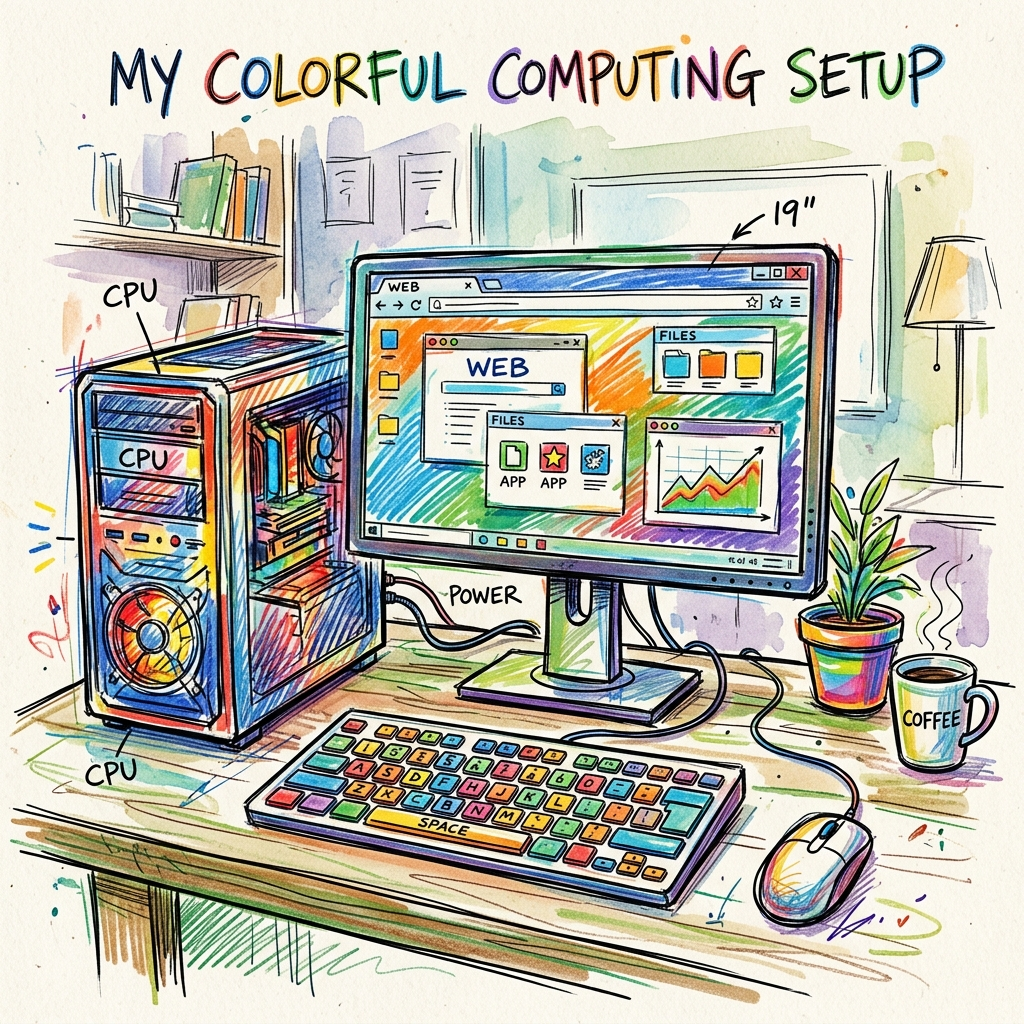
\includegraphics[width=0.9\linewidth]{vokab_300dpi/computer.png} \\
            \small\textit{De Computer (L'ordinateur / The computer)}
            \vspace{0.5cm}
        }}
    \end{minipage}
    
    \vspace{1.5em}
    
    \begin{minipage}[t]{0.48\textwidth}
        \centering
        \textbf{E Kino}
        \vspace{0.5em}
        \framebox{\parbox{0.9\linewidth}{\centering
            \vspace{0.5cm}
            
\includegraphics[width=0.9\linewidth]{vokab_300dpi/kino.png} \\
            \small\textit{De Kino (Le cinéma / The cinema)}
            \vspace{0.5cm}
        }}
    \end{minipage}
    \hfill
    \begin{minipage}[t]{0.48\textwidth}
        \centering
        \textbf{Eng Zäitschrëft}
        \vspace{0.5em}
        \framebox{\parbox{0.9\linewidth}{\centering
            \vspace{0.5cm}
            
\includegraphics[width=0.9\linewidth]{vokab_300dpi/zaitschreft.png} \\
            \small\textit{D'Zäitschrëft (Le magazine / The magazine)}
            \vspace{0.5cm}
        }}
    \end{minipage}
\end{center}
